\documentclass{ximera}
\author{Bart Snapp}
\newcommand{\RR}{\mathbb R}
\renewcommand{\d}{\,d}
\newcommand{\dd}[2][]{\frac{d #1}{d #2}}
\renewcommand{\l}{\ell}
\newcommand{\ddx}{\frac{d}{dx}}
\newcommand{\dfn}{\textbf}
\newcommand{\eval}[1]{\bigg[ #1 \bigg]}


\outcome{Understand how to break up fractions.}
\outcome{Recognize integrals that are good candidates for the method of partial fractions.}
\outcome{Use long-division to simplify rational expressions.}
\outcome{Find the coefficients of partial fraction decomposition.}
\outcome{Use partial fractions to integrate functions.}

\title[Dig-In:]{Rational functions}

\begin{document}
\begin{abstract}
We discuss an approach that allows us to integrate rational functions.
\end{abstract}
\maketitle

\section{Basics of polynomial and rational functions}

In this course, we are attempting to learn to work with as many
functions as possible. A basic class of functions are \textit{polynomial functions}:

\begin{definition}
  A \dfn{polynomial function} in the variable $x$ is a function
  which can be written in the form
  \[
  f(x) = a_nx^n + a_{n-1}x^{n-1} + \dots + a_1 x + a_0
  \]
  where the $a_k$'s are all constants (called the \dfn{coefficients})
  and $n$ is a whole number (called the \dfn{degree} when $n\ne
  0$). The domain of a polynomial function is $(-\infty,\infty)$.
\end{definition}

\begin{question}
  Which of the following are polynomial functions?
  \begin{selectAll}
    \choice[correct]{$f(x) = 0$}
    \choice[correct]{$f(x) = 3x+1$}
    \choice{$f(x) = x^{1/2}-x +8$}
    \choice{$f(x) = -4x^{-3}+5x^{-1}+7-18x^2$}
    \choice[correct]{$f(x) = (x+1)(x-1)+e^x - e^x $}
    \choice{$f(x) = \frac{x^2 - 3x + 2}{x-2}$}
    \choice[correct]{$f(x) = x^7-32x^6-\pi x^3+45/84$}
  \end{selectAll}
\end{question}

As we will see, there is a fact about polynomials that is of critical
importance for this section:
\begin{quote}
  \textbf{Polynomials are equal as functions if and only if their
    coefficients are equal.}
\end{quote}

\begin{question}
  Given two polynomials equal as functions:
  \[
  6x^5+a_4 x^4 -x^2 + a_0 = a_5 x^5 - 24 x^4 + a_3 x^3 + a_2 x^2 - 5
  \]
  What are $a_0$, $a_1$, $a_2$, $a_3$, $a_4$, $a_5$?
  \begin{prompt}
    \begin{itemize}
    \item $a_0 = \answer{-5}$
    \item $a_1 = \answer{0}$
    \item $a_2 = \answer{-1}$
    \item $a_3 = \answer{0}$
    \item $a_4 = \answer{-24}$
    \item $a_5 = \answer{6}$
    \end{itemize}
  \end{prompt}
\end{question}

In the world of mathematics, polynomials are a generalization of
``integers,'' and rational numbers are fractions of integers. This
brings us to our next definition:

\begin{definition}
  A \dfn{rational function} in the variable $x$ is a function the form
  \[
  f(x) = \frac{p(x)}{q(x)}
  \]
  where $p$ and $q$ are polynomial functions. The domain of a rational
  function is all real numbers except for where the denominator is
  equal to zero.
\end{definition}

\begin{question}
  Which of the following are rational functions?
  \begin{selectAll}
    \choice[correct]{$f(x) = 0$}
    \choice[correct]{$f(x) = \frac{3x+1}{x^2-4x+5}$}
    \choice{$f(x)=e^x$}
    \choice{$f(x)=\frac{\sin(x)}{\cos(x)}$}
    \choice[correct]{$f(x) = -4x^{-3}+5x^{-1}+7-18x^2$}
    \choice{$f(x) = x^{1/2}-x +8$}
    \choice{$f(x)=\frac{\sqrt{x}}{x^3-x}$}
  \end{selectAll}
  \begin{feedback}
    All polynomials can be thought of as rational functions.
  \end{feedback}
\end{question}


\section{Denominators with distinct linear factors}


We are already skilled at working with polynomials, we can
differentiate and integrate any polynomial function. Being able to
integrate \textit{any} rational function is the next logical step in
our (rather ambitious) quest to integrate \textit{all}
functions. Let's dig right in with an example.

\begin{example}
  Compute:
  \[
  \int \frac{1}{x^2-1} \d x
  \]
  \begin{explanation}
    We will suppose that there are numbers $A$ and $B$ such that
    \[
    \frac{A}{x-1} + \frac{B}{x+1} = \frac{1}{x^2-1}.
    \]
    Clearing denominators, we find
    \[
    A\answer[given]{(x+1)} + B\answer[given]{(x-1)} = 1.
    \]
    Expanding the left-hand side, we find a polynomial equal (as a
    function!) to the constant polynomial $1$
    \[
    (A+ B)x + (A-B) = 1
    \]
    Since \textbf{polynomials are equal as functions if and only if
      their coefficients are equal}, we may rewrite this as
    \textbf{two} equations:
    \begin{align*}
      \answer[given]{A+B} &= 0 &\text{(the coefficients for $x$)}\\
      \answer[given]{A-B} &= 1 &\text{(the coefficients for the constant)}
    \end{align*}
    Solving these three equations for $A$ and $B$ we find
    \begin{itemize}
    \item $A = \answer[given]{1/2}$,
    \item $B = \answer[given]{-1/2}$.
    \end{itemize} 
    From this we can now rewrite our integral as
    \begin{align*}
      \int \frac{1}{x^2-1} \d x &=  \int \frac{1/2}{x-1} + \frac{-1/2}{x+1} \d x\\
      &= (1/2)\ln|x-1| + (-1/2)\ln|x+1|+ K.
    \end{align*}
  \end{explanation}
\end{example}

What we have seen is part of a general technique of integration called
``partial fractions''\index{partial fractions} that, in principle,
allows us to integrate any rational function.

\subsection{The general technique for distinct linear factors}

Suppose you wish to compute
\[
\int \frac{p(x)}{q(x)} \d x
\]
where $p$ and $q$ are both polynomial functions, the degree of $p$ is
less than the degree of $q$, and $q$ factors into $n$
\textbf{distinct} linear factors:
\[
q(x) = (x-r_1) (x-r_2) \cdots (x-r_n),
\]
then we can \textbf{always} write
\[
\frac{p(x)}{q(x)}  = \frac{A_1}{(x-r_1)} + \frac{A_2}{(x-r_2)} + \cdots + \frac{A_n}{(x-r_n)}. 
\]
The right-hand side of the equation above is easy to antidifferentiate,
as we can integrate it term-by-term and
\[
\int \frac{A_k}{(x-r_k)} \d x = A \ln(x-r_k) + K,
\]
hence
\[
\int \frac{p(x)}{q(x)} \d x = \sum_{k=1}^n A_k \ln|x-r_k| +K.
\]








\section{Denominators with repeated linear factors}

Here we work as we did before, except we add an extra variable for
each of the repeated factors. Let's do an example.

\begin{example}
  Compute:
  \[
  \int \frac{1}{(x-1)(x+2)^2} \d x
  \]
  \begin{explanation}
    We will suppose that there are numbers $A$, $B$, and $C$ such that
    \[
    \frac{A}{x-1} + \frac{B}{x+2} + \frac{C}{(x+2)^2} = \frac{1}{(x-1)(x+2)^2}
    \]
    Clearing denominators, we find
    \[
    A\answer[given]{(x+2)^2} + B\answer[given]{(x-1)(x+2)} + C\answer[given]{(x-1)} = 1.
    \]
    Expanding the left-hand side, we find a polynomial equal (as a
    function!) to the constant polynomial $1$
    \[
    (A+B)x^2 + (4A+B+C)x + (4A-2B-C) = 1
    \]
    Since \textbf{polynomials are equal as functions if and only if
      their coefficients are equal}, we may rewrite this as
    \textbf{three} equations:
    \begin{align*}
      \answer[given]{A+B} &= 0 &\text{(the coefficients for $x^2$)}\\
      \answer[given]{4A+B+C} &= 0 &\text{(the coefficients for $x$)}\\
      \answer[given]{4A-2B-C} &= 1 &\text{(the coefficients for the constant)}
    \end{align*}
    Solving these three equations for $A$, $B$ and $C$ we find
    \begin{itemize}
    \item $A = \answer[given]{1/9}$,
    \item $B = \answer[given]{-1/9}$,
    \item $C = \answer[given]{-1/3}$.
    \end{itemize}
    From this we can now rewrite our integral as
    \begin{align*}
      \int&\frac{1}{(x-1)(x+2)^2}\d x= \int \frac{1/9}{x-1}+ \frac{-1/9}{x+2} + \frac{-1/3}{(x+2)^2}\d x\\
      &= \int \frac{1/9}{x-1}\d x + \int \frac{-1/9}{x+2}\d x + \int \frac{-1/3}{(x+2)^2}\d x,\\
      &= \frac{1}{9}\ln|x-1| -\frac{1}{9}\ln|x+2| +\frac{1}{3(x+2)}+K.
    \end{align*}
  \end{explanation}
\end{example}



\subsection{The general technique for repeated linear factors}

Suppose you wish to compute
\[
\int \frac{p(x)}{q(x)} \d x
\]
where $p$ and $q$ are both polynomial functions, the degree of $p$ is
less than the degree of $q$, and $q$ factors into $n$
\textbf{repeated} linear factors:
\[
q(x) = (x-r)^n,
\]
then we can \textbf{always} write
\[
\frac{p(x)}{q(x)}  = \frac{A_1}{(x-r)} + \frac{A_2}{(x-r)^2} + \cdots + \frac{A_n}{(x-r)^n}. 
\]
The right-hand side of the equation above is easy to
antidifferentiate, as we can integrate it term-by-term and
\begin{align*}
  \int \frac{A_1}{(x-r)} \d x &= A_1 \ln|x-r| + K,\\
  \int \frac{A_k}{(x-r)^k} \d x &= \frac{A_k}{(1-k)(x-r)^{k-1}}+ K, &\text{(if $k>1$)}
\end{align*}
hence
\[
\int \frac{p(x)}{q(x)} \d x = A_1 \ln|x-r|  + \sum_{k=2}^n \frac{A_k}{(1-k)(x-r)^{k-1}} + K.
\]






\section{Denominators with distinct irreducible quadratic factors}

Here is a fact about polynomials:

\begin{theorem}[The Fundamental Theorem of Algebra]\index{Fundamental Theorem of Algebra}
  Every polynomial of the form
  \[
  a_n x^n + a_{n-1} x^{n-1} + \dots + a_1 x + a_0
  \]
  where the $a_i$'s are real (or even complex!) numbers and $a_n \ne 0$ has exactly
  $n$ (possibly repeated) complex roots.
\end{theorem}

Remember, a \dfn{root} is where a polynomial is zero. The theorem
above is a deep fact of mathematics. The great mathematician Gauss
%(spelled Gau\ss\ for fancy people)
proved the theorem in 1799 for his doctoral thesis. This fact can be
used to show the following:
\begin{quote}
  \textbf{Every polynomial function will factor as a product of linear
    terms and irreducible quadratic terms over the real numbers.}
\end{quote}

So now let's work an example where the denominator of our rational
function has distinct quadratic factors.

\begin{example}
  Compute:
  \[
  \int\frac{7x^2+31x+54}{(x+1)(x^2+6x+11)}\d x
  \]
  \begin{explanation}
    We will suppose that there are numbers $A$, $B$, and $C$ such that
    \[
    \frac{A}{x+1} + \frac{Bx+C}{x^2+6x+11} = \frac{7x^2+31x+54}{(x+1)(x^2+6x+11)}.
    \]
    Clearing denominators, we find
    \[
    \left(\answer[given]{x^2+6x+11}\right)A + (Bx+C)\left(\answer[given]{x+1}\right) = 7x^2+31x+54.
    \]
    Expanding the left-hand side, we find a polynomial equal (as a
    function!) to the polynomial $7x^2+31x+54$
    \[
    (A+B)x^2 + (6A+B+C)x + (11A+C) = 7x^2+31x+54.
    \]
    Since \textbf{polynomials are equal as functions if and only if
      their coefficients are equal}, we may rewrite this as
    \textbf{three} equations:
    \begin{align*}
      \answer[given]{A+B} &= 7 &\text{(the coefficients for $x^2$)}\\
      \answer[given]{6A+B+C} &= 31 &\text{(the coefficients for $x$)}\\
      \answer[given]{11A+C} &= 54 &\text{(the coefficients for the constant)}
    \end{align*}
    Solving these three equations for $A$, $B$ and $C$ we find
    \begin{itemize}
    \item $A = \answer[given]{5}$,
    \item $B = \answer[given]{2}$,
    \item $C = \answer[given]{-1}$.
    \end{itemize}
    From this we can now rewrite our integral as
    \[
    \int\frac{7x^2+31x+54}{(x+1)(x^2+6x+11)}\d x = \int\frac{5}{x+1} + \frac{2x-1}{x^2+6x+11} \d x\\
    \]
    The first term of this new integrand is easy to evaluate. We find
    \[
    \int \frac{5}{x+1} \d x = 5\ln|x+1|+K.
    \]
    The second term is not hard, but takes several steps and uses
    substitution techniques.

    The integrand $\frac{2x-1}{x^2+6x+11}$ has a quadratic in the
    denominator and a linear term in the numerator. This leads us to
    try substitution. Let
    \begin{align*}
      g &= x^2+6x+11,\\
      \d g  &= (2x+6)\d x.
    \end{align*}
    However, the numerator is $2x-1$, not $2x+6$! We can bypass this
    difficulty by adding ``$0$'' in the form of ``$7-7$.''
\begin{align*}
  \frac{2x-1}{x^2+6x+11} &= \frac{2x-1+7-7}{x^2+6x+11} \\
  &= \frac{2x+6}{x^2+6x+11} - \frac{7}{x^2+6x+11}.
\end{align*}
We can now integrate the first term with substitution, leading to
\[
\int \frac{2x+6}{x^2+6x+11} \d x = \ln|x^2+6x+11| + K.
\]
The final term can be integrated using arctangent. First, complete the
square in the denominator:
\[
\frac{7}{x^2+6x+11} = \frac{7}{(x+3)^2+2}.
\]
then use a substitution of $g = x+3$ to find
\[
\int \frac{7}{x^2+6x+11}\d x = \frac{7}{\sqrt{2}}\arctan\left(\frac{x+3}{\sqrt{2}}\right)+K.
\]
Let's start at the beginning and put all of the steps together.
\begin{align*}
  \int&\frac{7x^2+31x+54}{(x+1)(x^2+6x+11)}\d x \\
  &= \int\left(\frac{5}{x+1} + \frac{2x-1}{x^2+6x+11}\right)\d x
\end{align*}
breaking this integral up we find
\begin{align*}
  = \int\frac{5}{x+1}\d x  &+ \int\frac{2x+6}{x^2+6x+11}\d x\\
  &-\int\frac{7}{x^2+6x+11}\d x
\end{align*}
and antidifferentiating we find
\[
  = 5\ln|x+1|+ \ln|x^2+6x+11|-\frac{7}{\sqrt{2}}\arctan\left(\frac{x+3}{\sqrt{2}}\right)+K.
\]
  \end{explanation}
\end{example}


\subsection{The general technique for distinct quadratic factors}

Suppose you wish to compute
\[
\int \frac{p(x)}{q(x)} \d x
\]
where $p$ and $q$ are both polynomial functions, the degree of $p$ is
less than the degree of $q$, and $q$ factors into $n$
\textbf{distinct} irreducible quadratic factors:
\[
q(x) = (a_1x^2 + b_1 x + c_1) (a_2x^2 + b_2 x + c_2)\cdots  (a_nx^2 + b_n x + c_n) 
\]
then we can \textbf{always} write
\[
\frac{p(x)}{q(x)}  = \frac{A_1x+B_1}{a_1x^2 + b_1 x + c_1} + \cdots + \frac{A_nx+B_n}{a_nx^2 + b_n x + c_n}. 
\]
The right-hand side of the equation can be antidifferentiated, though it is not always ``easy.''







\section{Denominators with repeated quadratic factors}

For completeness sake, we will work a problem with repeated quadratic factors.

\begin{example}
  Compute
  \[
  \int \frac{1}{x^5 + 2x^3  + x}\d x
  \]
  \begin{explanation}
    Start by factoring the denominator
    \[
    x^5 + 2x^3  + x = x(x^2+1)^2.
    \]
    We will suppose that there are numbers $A$, $B$, $C$, $D$, and $E$
    such that
    \[
    \frac{A}{x} + \frac{Bx+C}{x^2+1} + \frac{Dx+E}{(x^2+1)^2} = \frac{1}{x(x^2+1)^2}.
    \]
    Clearing denominators, we find
    \[
    A\answer[given]{(x^2+1)^2} + (Bx+C)\answer[given]{(x^3+x)}+ (Dx+E)\answer[given]{(x)} = 1
    \]
    Expanding the left-hand side, we find a polynomial equal (as a
    function!) to the constant $1$.
    \[
    (A+B)x^4 +  Cx^3 + (2A+B+D)x^2 + (C+E)x + A = 1.
    \]
    Since \textbf{polynomials are equal as functions if and only if
      their coefficients are equal}, we may rewrite this as
    \textbf{five} equations:
    \begin{align*}
      \answer[given]{A+B} &= 0 &\text{(the coefficients for $x^4$)}\\
      \answer[given]{C} &= 0 &\text{(the coefficients for $x^3$)}\\
      \answer[given]{2A+B+D} &= 0 &\text{(the coefficients for $x^2$)}\\
      \answer[given]{C+E} &= 0 &\text{(the coefficients for $x$)}\\
      \answer[given]{A} &= 1 &\text{(the coefficients for the constant)}
    \end{align*}
    Solving these three equations for $A$, $B$, $C$, $D$, and $E$ we find
    \begin{itemize}
    \item $A = \answer[given]{1}$,
    \item $B = \answer[given]{-1}$,
    \item $C = \answer[given]{0}$,
    \item $D = \answer[given]{-1}$,
    \item $E = \answer[given]{0}$.
    \end{itemize}
    From this we can now rewrite our integral as
    \[
    \int \frac{1}{x^5 + 2x^3  + x}\d x =\int \frac{1}{x} + \frac{-x}{x^2+1} + \frac{-x}{(x^2+1)^2}\d x
    \]
    Each term of this new integrand is easy to evaluate, write
    \begin{align*}
      \int \frac{1}{x} \d x &= \ln|x| + K,\\
      \int \frac{-x}{x^2+1} \d x &= \frac{-\ln|x^2+1|}{2} +K,\\
      \int \frac{-x}{(x^2+1)^2} \d x &= \frac{1}{2(x^2+1)}+K.
    \end{align*}
    So
    \begin{align*}
    \int &\frac{1}{x^5 + 2x^3  + x}\d x \\
    &=\ln|x| + \frac{-\ln|x^2+1|}{2} + \frac{1}{2(x^2+1)}+K.
    \end{align*}
  \end{explanation}
\end{example}



\subsection{The general technique for repeated quadratic factors}
Suppose you wish to compute
\[
\int \frac{p(x)}{q(x)} \d x
\]
where $p$ and $q$ are both polynomial functions, the degree of $p$ is
less than the degree of $q$, and $q$ factors into $n$
\textbf{distinct} irreducible quadratic factors:
\[
q(x) = (ax^2 + b x + c)^n 
\]
then we can \textbf{always} write
\[
\frac{p(x)}{q(x)}  = \frac{A_1x+B_1}{ax^2 + bx + c} + \frac{A_2x+B_2}{(ax^2 + bx + c)^2} + \cdots + \frac{A_nx+B_n}{(ax^2 + b x + c)^n}. 
\]
The right-hand side of the equation can be antidifferentiated, though it is not always ``easy.''


\section{Reducing rational functions}

When computing
\[
\int \frac{p(x)}{q(x)} \d x
\]
all of the techniques above rely on the fact that the degree of $p$ is
less than the degree of $q$. What if this is not the case? Use
\index{long-division}long-division.

\begin{example}
  Compute:
  \[
  \int \frac{x^3+1}{x^2-1} \d x
  \]
  \begin{explanation}
    We start by using long-division to reduce the numerator:
    \begin{image}[2in]
      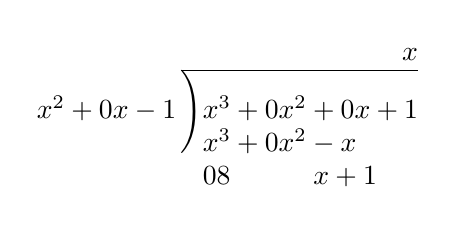
\begin{tikzpicture}[]
        \node at (0,0) {
          $x^2+0x-1\,\begin{array}[b]{@{}r@{}r} 
          x &\\ 
          \cline{1-1}
          \Bigg)\begin{array}[t]{@{}l@{}} x^3+0x^2+0x+1\\ 
            x^3+0x^2-x \\ 
            \divrule{0}{8}  ~~~~~~~~~x+1
          \end{array}
          \end{array}
          $
        };
      \end{tikzpicture}
    \end{image}
    Now our integral becomes
    \[
    \int \frac{x^3+1}{x^2-1}\d x = \int x+ \frac{x+1}{x^2-1}\d x
    \]
    From here, we can use our techniques from before to complete the
    computation, or we can note more simply that 
    
    \[
    \frac{x+1}{x^2-1}=\frac{x+1}{(x+1)(x-1)} = \frac{1}{x-1}.
    \]
  \end{explanation}
\end{example}
    


As with many other problems in calculus, it is important to remember
that one is not expected to ``see'' the final answer immediately after
seeing the problem. Rather, given the initial problem, we break it
down into smaller problems that are easier to solve. The final answer
is a combination of the answers of the smaller problems.
\end{document}
